\chapter{Herramientas Numéricas} \label{cap:numerico}

En este capítulo se da una breve descripción de las herramientas numéricas utilizadas: Xcompact3D y OSMC. Xcompact3D resuelve las ecuaciones de Navier-Stokes junto a la ecuación de transporte de un escalar, brindando la capacidad de resolver en forma eficiente y precisa flujos turbulentos en canales rectangulares usando una grilla cartesiana simple; además, es una herramienta popular en el ámbito de la investigación básica y aplicada. Una descripción completa de la misma puede encontrarse en \url{https://www.incompact3d.com/}.

Por su parte, OSMC se emplea para resolver el problema de autovalores y autofunciones detallado en la sección \ref{sec:estabilidad}. El mismo utiliza el método espectral de Colocación de la Matriz de Chebyshev transformando el problema original a un problema autovalores y autovectores. Esta herramienta fue desarrollada por Pablo Szuban \cite{szuban2023} en el grupo de Mecánica Computacional (MECOM-CAB). 


\section{Xcompact3D (XC3D)}

Comprender, predecir y controlar los flujos turbulentos es crucial, y a la vez, un factor relevante en la industria, no en vano sigue siendo uno de los desafíos más complejos en investigación. Además, el diseño de numerosos sistemas de ingeniería e industriales, así como la evaluación de su impacto ambiental, depende de cuantificar con precisión el comportamiento turbulento de los flujos.

Si bien las ecuaciones de Navier-Stokes constituyen el modelo matemático de referencia para describir la dinámica de un flujo turbulento, su resolución es especialmente exigente debido al carácter caótico y multiescala de la turbulencia \cite{pope2001turbulent}. Las escalas relevantes abarcan varios órdenes de magnitud y demandan elevados recursos de cómputo y memoria. El notable incremento en las últimas dos décadas en la capacidad computacional ha impulsado el uso de simulaciones de alta fidelidad; en particular, las simulaciones DNS\footnote{Simulaciones numéricas en las que se resuelve la gran mayoría de las escalas turbulentas.} se han consolidado como una herramienta clave para la predicción de flujos y se han convertido, junto al CFD\footnote{\textit{Computational Fluid Dynamics}}, en un complemento esencial de la teoría y el experimento.

En este trabajo se estudian el flujo de un fluido y la transferencia de calor en régimen turbulento con convección mixta, así como la transición laminar-turbulenta temporal, mediante simulaciones numéricas directas. Ello exige resolver las ecuaciones de Navier-Stokes y de transporte de un escalar, acopladas entre sí, con alta precisión numérica y eficiencia computacional. Para este fin se emplea Xcompact3D\footnote{Abreviado en este trabajo como XC3D}, una herramienta numérica implementada en Fortran 90/95 orientada a arquitecturas basadas en CPU y a la Computación de Alto Desempeño (HPC). XC3D evoluciona a partir del \textit{flow solver} Incompact3D, desarrollado originalmente en Francia a mediados de los años noventa, y posteriormente portado a sistemas HPC a comienzos de la década de 2010.

Algunas características distintivas de XC3D son:
\begin{itemize}
\item Implementa diversos flujos canónicos, entre ellos el flujo en dominios tipo caja con geometría cartesiana, adecuados para los objetivos de este trabajo.
\item Es una herramienta de código abierto, con documentación en \href{https://xcompact3d.readthedocs.io/en/latest/}{Read the Docs} y código disponible en \href{https://github.com/xcompact3d}{GitHub}.
\item Presenta alta eficiencia y escalabilidad, con dependencia mínima de bibliotecas externas (solo requiere una biblioteca basada en MPI\footnote{\textit{Message Passing Interface}. Más información en \href{https://www.mpi-forum.org/}{MPI-Forum}.}: \textit{2D Decomp \& FFT} \cite{li20102decomp}, \cite{laizet2011incompact3d}).
\item Utiliza grilla o malla uniforme en dos direcciones (X y Z) y uniforme o refinada en la dirección Y (coordenada
pensada para paredes).
\item Ofrece una compilación ágil y sencilla mediante un único \textit{Makefile}; los parámetros numéricos de la simulación (tamaño del dominio, número de nodos de la grilla, etc.) pueden ajustarse sin recompilar.
\end{itemize}


\begin{figure}[H]
 \centering
    \subfloat[]{
    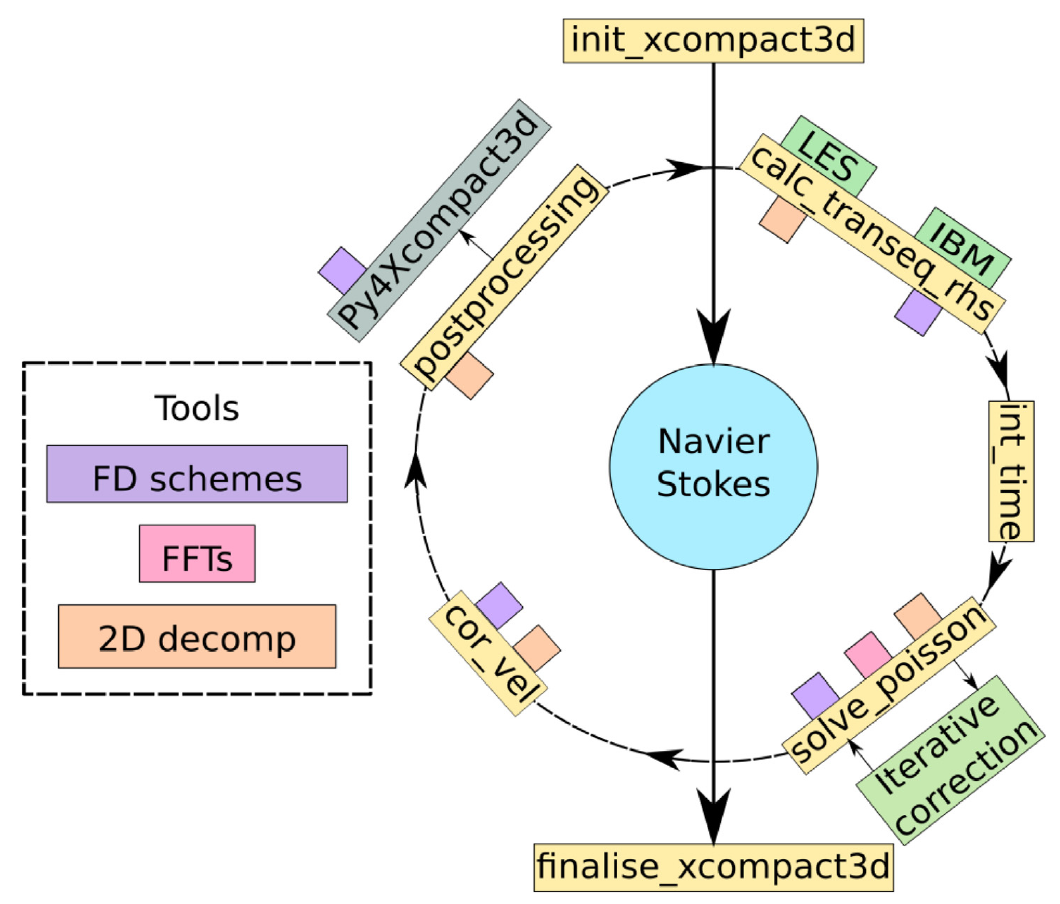
\includegraphics[width=0.49\textwidth]{figures/cap3/xc3d_architecture.png}
    	\label{fig:xc3d_archi}}  
    
    \subfloat[]{
    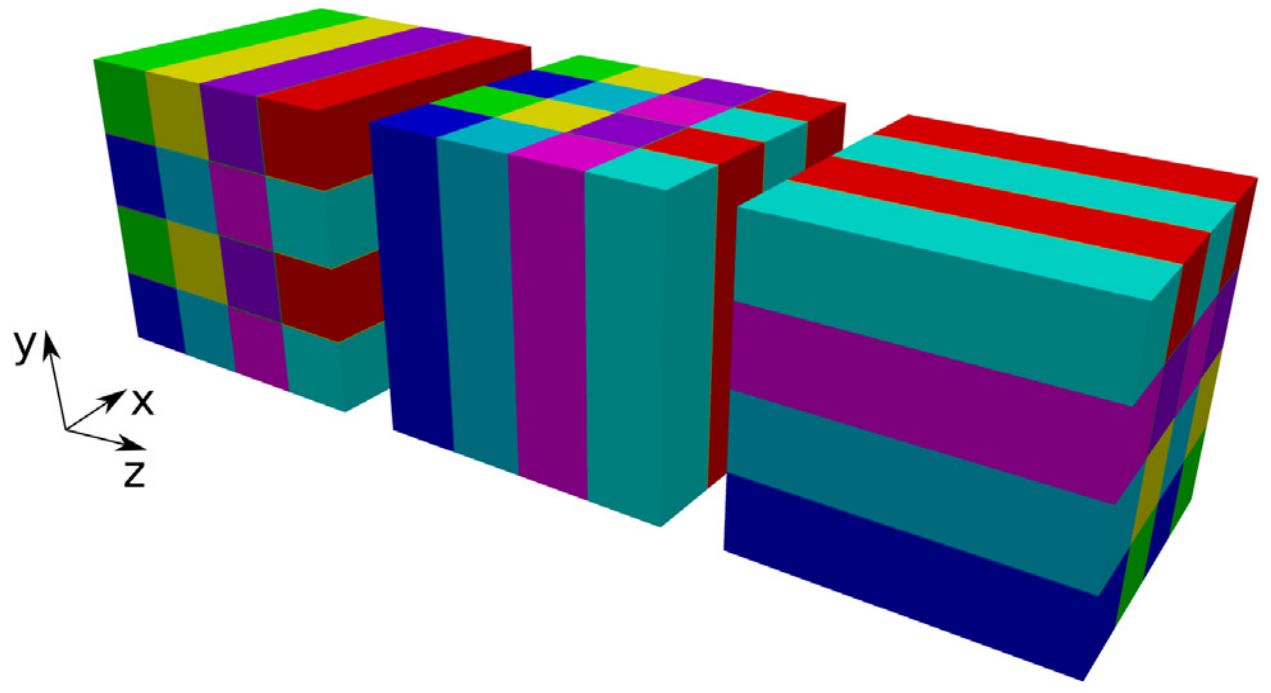
\includegraphics[width=0.49\textwidth]{figures/cap3/2d_decomp.png}
    	\label{fig:2d_decomp}}
 \caption{\textbf{(a)} Diagrama de la arquitectura de software de Xcompact3D. \textbf{(b)} Descomposición en lápices 2D utilizando 4 $\times$ 4 procesadores, representando los mismos en direcciones X, Y y Z respectivamente. Imágenes tomadas de \cite{bartholomew2020xcompact3d}.} 
 \label{fig:xc3d}
\end{figure}

El objetivo de las próximas subsecciones es ofrecer al lector una visión general de la lógica algorítmica de la herramienta numérica; se trata de un esquema conceptual a grandes rasgos, no de una descripción formal y rigurosa.

\subsection{Ecuaciones de gobierno}

Xcompact3D resuelve numéricamente las ecuaciones de Navier-Stokes para flujo incompresible junto con la ecuación de transporte de temperatura, acopladas entre sí mediante el término de fuerza boyante en la ecuación de momento. Las ecuaciones se expresan en forma adimensional en \ref{eq:sistem2} donde se omiten los superíndices ``*'' a fin de simplificar la notación. {\linebreak}Obsérvese que si bien las ecuaciones están en consonancia con lo expuesto en el Capítulo \ref{cap:modelo}, no son exactamente las mismas. No obstante, estas ligeras diferencias no resultan relevantes en la explicación del método numérico.

\begin{equation}
\begin{aligned}
&\nabla \cdot \mathbf{u} = 0 \\
& \frac{\partial \mathbf{u}}{\partial t} = -\nabla \text{p} \underbrace{- (\mathbf{u} \cdot \nabla)\mathbf{u} + \frac{1}{\text{Re}} \nabla^2 \mathbf{u} + \mathbb{A} \hspace{0.5mm} \theta \hspace{0.5mm} \mathbf{e}_g + \mathbf{f} }_{\textbf{RHS}_{1}} \\
& \frac{\partial \theta}{\partial t} = \underbrace{- \mathbf{u} \cdot \nabla \theta + \frac{1}{\text{Re} \text{Pr}} \nabla^2 \theta + \mathbb{B} \hspace{0.5mm} u_x }_{\textbf{RHS}_2} \\
\end{aligned}
\label{eq:sistem2}
\end{equation}
En las ecuaciones precedentes: $\text{p}(\mathbf{x},t)$, $\mathbf{u}(\mathbf{x},t)$, $\theta(\mathbf{x},t)$
son los campos de presión, velocidad y temperatura respectivamente; $\mathbf{x} = (x,y,z)$ es el vector de coordenadas y $t$ el tiempo; Re y Pr son los números adimensionales de Reynolds y Prandtl respectivamente; $\mathbb{A}$ y $\mathbb{B}$ son constantes. Dependiendo de la forma adimensional considerada, $\mathbb{A}$ y $\mathbb{B}$ pueden ser diferentes. Por ejemplo, tomando $\mathbb{A}=\text{Ri} / (\text{Re} \hspace{0.5mm} \text{Pr})$ y $\mathbb{B}=1$  se obtiene la forma adimensional de las ecuaciones \ref{eq:gob_system_adim}. La fuerza volumétrica $\mathbf{f}(\mathbf{x},t)$ es usada cuando se sumerge un cuerpo sólido dentro del dominio computacional (\textit{Immersed Boundary Method} \cite{peskin2002immersed}) o para otros usos según sea requerido.


\subsection{Esquemas de diferencias finitas de alto orden}

Las ventajas de los esquemas de alto orden para DNS/LES frente a los esquemas \linebreak convencionales de bajo orden están plenamente reconocidas actualmente, especialmente por su capacidad de capturar con precisión un rango más amplio de escalas turbulentas para una resolución espacial dada. Por otro lado, los métodos espectrales estándar basados en representaciones de Fourier o de Chebyshev proporcionan soluciones muy precisas y eficientes de las ecuaciones de Navier-Stokes, aunque con severas restricciones en su aplicabilidad. Por su parte, los esquemas compactos de diferencias finitas de alto orden \cite{laizet2009high} se aproximan a la precisión de los métodos espectrales y permiten mayor flexibilidad en la selección de condiciones de contorno (en XC3D es posible usar condiciones\footnote{Recuérdese que en este trabajo se utiliza la aproximación MBC para imponer la condición de borde térmica (véase Sección \ref{sec:descripcion}), ya que ha sido ampliamente evaluada y utilizada en el grupo de trabajo.} periódicas, de Dirichlet y de Neumann). Aunque los esquemas compactos son implícitos en el espacio, resultan muy competitivos en términos de eficiencia computacional. En particular, nuestras simulaciones emplean esquemas compactos de sexto orden para la discretización de los términos convectivo y difusivo.

\subsection{Avance temporal} \label{sec:time-ava}

El campo de flujo y el campo escalar se inicializan ya sea con una condición inicial (\texttt{init\_xcompact3d} en la Figura \ref{fig:xc3d_archi}) o cargando un archivo \textit{restart}. Las ecuaciones de Navier-Stokes se avanzan en el tiempo mediante un método de paso fraccionado (o proyección) implementado en tres etapas lógicas: (i) evaluación del lado derecho y \textit{predictor}, (ii) resolución de la ecuación de Poisson para la presión  e imposición de incompresibilidad y (iii) corrección \linebreak  de la velocidad y la temperatura.  En la Figura \ref{fig:xc3d_archi} se presenta una visión general de la arquitectura modular de Xcompact3D \cite{bartholomew2020xcompact3d}. Las principales funcionalidades se separan en los módulos: \texttt{calc\_transeq\_rhs}, \texttt{int\_time}, \texttt{solve\_poisson}, \texttt{cor\_vel} y \texttt{postprocessing}. Los tres primeros corresponden a la resolución de las ecuaciones de gobierno, mientras que el último corresponde a la etapa de postprocesamiento de los datos obtenidos:


\begin{enumerate}
\item[\textbf{I}] \texttt{calc$\_$transeq$\_$rhs} $\rightarrow$ \texttt{int$\_$time}: predictor $\mathbf{u}^{\dagger \dagger}$ \\
Primero, se evalúan numéricamente los términos del lado derecho (\textbf{RHS}$_1$) de la ecuación de momento y se integran en el tiempo (una vez discretizados en el espacio) empleando, por ejemplo, esquemas de Runge-Kutta o Adams-Bashforth para obtener la velocidad intermedia $\mathbf{u}^{\dagger}$:

\begin{equation}
\frac{\mathbf{u}^{\dagger} - \mathbf{u}^k}{\Delta t} = \textbf{RHS}_1^k - c_k \nabla \widetilde{\text{p}}^k , 
\end{equation}
donde $c_k$ es un coeficiente conocido y $k$ el índice para los subpasos de tiempo \linebreak $k=1,...,n_k$; con $t_1=t_n$ y $t_{n_k}=t_{n+1}$ ($\Delta t = t_{n+1} - t_{n}$). La presión se expresa \linebreak como su valor promediado en el tiempo en un subpaso dado ($c_k \Delta t$) indicado con una tilde $\widetilde{(\text{.})}$. Por conveniencia algebraica y para limpiar el lado derecho de la ecuación de \linebreak Poisson de los pasos posteriores, puede definirse un campo intermedio $\mathbf{u}^{\dagger \dagger}$ que ``remueve'' la presión promedio usada en el predictor:

\begin{equation}
\frac{\mathbf{u}^{\dagger \dagger} - \mathbf{u}^{\dagger}}{\Delta t} = c_k \nabla \widetilde{\text{p}}^k  
\end{equation}
Con esta reordenación, $\mathbf{u}^{\dagger \dagger}$ sólo contiene los aportes no asociados a la presión previa:

\begin{equation}
\frac{\mathbf{u}^{\dagger \dagger} - \mathbf{u}^{k}}{\Delta t} = \textbf{RHS}_1^k \text{.}  
\end{equation}

\item[\textbf{II}] \texttt{solve\_poisson}: presión de proyección $\widetilde{p}^{k+1}$ \\
Se impone la incompresibilidad al final del paso:
	
\begin{equation}
\nabla \cdot \mathbf{u}^{k+1} = 0.
\label{eq:incomp}
\end{equation}
Tomando la divergencia de la corrección (véase ecuación \ref{eq:correccion}) y utilizando la ecuación \ref{eq:incomp}, se obtiene la ecuación de Poisson para la presión de proyección:

\begin{equation}
\nabla^2 \widetilde{\text{p}}^{k+1} = \frac{1}{c_k \Delta t} \nabla \cdot \mathbf{u}^{\dagger \dagger},
\end{equation}
donde $\widetilde{\text{p}}^{k+1}= \frac{1}{c_k \Delta t} \int^{t_{k+1}}_{t_k} \text{p} \hspace{0.5mm} dt$. 

Para la presión se aplican típicamente condiciones de borde de Neumann homogéneas (compatibles con la proyección). Por otro lado, las condiciones en la velocidad (por ejemplo, no deslizamiento) se aplican al predictor.

	\item[\textbf{III}]  \texttt{cor\_vel}: corrección solenoidal $\mathbf{u}^{k+1}$ \\
	Finalmente, se corrige la velocidad intermedia con el gradiente de la nueva presión para obtener
el campo solenoidal al final del paso de tiempo:

\begin{equation}
\frac{ \mathbf{u}^{k+1} - \mathbf{u}^{\dagger \dagger} }{\Delta t} = - c_k \nabla \widetilde{\text{p}}^{k+1} \text{.}
\label{eq:correccion}
\end{equation}

El término de la fuerza boyante no modifica la forma de la ecuación Poisson, sólo influye a través del predictor $\mathbf{u}^{\dagger \dagger}$ que genera. Adicionalmente, en el paso de tiempo actual $k$, se evalúa el lado derecho de la ecuación de transporte del escalar (\textbf{RHS}$_2$) empleando la velocidad calculada en el mismo paso, esto es:

\begin{equation}
\begin{aligned}
& \textbf{RHS}_2^k = - \mathbf{u}^{k} \cdot \nabla \theta^k + \frac{1}{\text{Re} \text{Pr}} \nabla^2 \theta^k + \mathbb{B} \hspace{0.5mm} u_x^{k}, \\
& \frac{\theta^{k+1} - \theta^{k}}{\Delta t} = \textbf{RHS}_2^k \text{.}
\end{aligned}
\end{equation}
Para la integración temporal de \textbf{RHS}$_2$ se emplea el mismo esquema utilizado en \textbf{RHS}$_1$.

\item[\textbf{IV}] \texttt{postprocessing} \\
Al final de cada paso de tiempo, el usuario puede decidir qué magnitudes almacenar y qué cantidades calcular (magnitudes estadísticas de primer orden, segundo orden, etc).

\end{enumerate}

En particular, en este trabajo, para la integración temporal de los términos \textbf{RHS}$_{1,2}$ se emplea el esquema Adams-Bashforth de orden 3.



\subsection{\textit{Solver} espectral de Poisson}

Como se menciona en la Sección \ref{sec:time-ava}, Xcompact3D avanza las ecuaciones de gobierno mediante el método de paso fraccionario, formando una ecuación de Poisson para la presión al tomar la divergencia de la ecuación de momento. Una de las principales originalidades de Xcompact3D es que la ecuación de Poisson se resuelve en el espacio espectral usando el concepto de números de onda modificados \cite{lele1992compact}, para los cuales las operaciones en el espacio físico son estrictamente equivalentes a las del espacio espectral. Esta estrategia directa, que evita el uso de costosas técnicas iterativas, no es nueva para condiciones de contorno periódicas y/o de deslizamiento libre del campo de velocidades \cite{schumann1976direct}. La misma ha sido implementada y validada para condiciones de Dirichlet combinadas con esquemas de diferencias finitas de alto orden \cite{laizet2009high}.

\subsection{Biblioteca \textit{2D Decomp $\&$ FFT}}

Los esquemas de diferencias finitas y el \textit{solver} espectral de Poisson empleados por \linebreak Xcompact3D se descomponen de forma natural en una serie de subproblemas unidimensionales. Por ello, resulta natural paralelizar el dominio computacional mediante una descomposición en “lápices”, como se ilustra en la Figura \ref{fig:2d_decomp}. Cada descomposición (en los ejes X, Y y Z, respectivamente) permite el cálculo independiente de derivadas, interpolaciones, etc. Las transposiciones globales para pasar de un lápiz a otro se realizan con comandos MPI. Más detalles sobre la estrategia de cómputo paralelo implementada en Xcompact3D pueden \linebreak encontrarse en \cite{laizet2011incompact3d}.



\section{Orr-Sommerfeld \textit{Mixed Convection} (OSMC)}

En el Capítulo \ref{cap:modelo}, empleando teoría de estabilidad lineal, considerando flujos laminares, y suponiendo las perturbaciones como ondas planas 3D (expresiones tipo \ref{eq:waves3d}) se arribó a un problema de autovalores y autofunciones generalizado, dado por la expresión \ref{eq:eigensistem-general}, con las condiciones de borde de la relación \ref{eq:eigensis-ci}. La herramienta numérica empleada para resolver este tipo de problemas es OSMC (por sus siglas, Orr-Somerfeld \textit{Mixed Convection}), desarrollada por Pablo Szuban como parte de su Proyecto Integrador de Ingeniería en el Instituto Balseiro \cite{szuban2023}. La herramienta numérica se implementó en lenguaje \textit{Python} utilizando las librerías \textit{NumPy} y \textit{SciPy}. La misma se encuentra disponible en GitHub: \href{https://github.com/Pato4184/OSMC-Repository}{OSMC-Repository}.

A continuación se dan los lineamientos detrás de la estrategia numérica utilizada. OSMC emplea el método numérico espectral conocido como ``Método de Colocación de la Matriz de Chebyshev'' \cite{moin2010fundamentals}. Esta estrategia busca transformar el problema de autovalores y autofunciones en uno de autovalores y autovectores. Los vectores solución son las amplitudes $\widehat{v_y}$, $\widehat{\varphi}$ y $\widehat{\eta}$ correspondientes a la frecuencia angular $\omega$ (autovalor asociado). Dado el sistema \ref{eq:eigensistem-general}, el flujo base laminar (Sección \ref{sec:fbase}) y las condiciones de borde asociadas, se discretiza la variable $y$ en el intervalo $\left[-1,1\right]$ en $N+1$ puntos de Chebyshev dados por la relación \ref{eq:cheb-points}. Lo siguiente es evaluar las funciones involucradas en dichos puntos, por ejemplo, para una función arbitraria $\xi$ se tienen los puntos $\xi_j = \xi(y_j)$; luego, se construye un polinomio interpolante de Lagrange $\mathcal{L}$ para $\xi$ , de grado $\leq N$, tal que $\mathcal{L}(y_j) = \xi_j$.

\begin{equation}
y_j = \cos \left( \frac{j \hspace{0.5mm} \pi}{N} \right), \quad j=0,1,...,N 
\label{eq:cheb-points}
\end{equation}

De esta manera, los valores de la derivada de $\xi$ en los puntos $y_j$ son equivalentes a aquellos valores de la derivada del polinomio interpolante en los mismos puntos. Si $\xi$ se transforma a un vector\footnote{Es decir, los elementos $\xi_j$ del vector $\vec{\xi}$ son tales que $\xi_j = \xi(y_j)$.} $\vec{\xi}$, entonces, se puede demostrar \cite{moin2010fundamentals}, que la derivada de la función evaluada en los puntos de Chebyshev es $\vec{\xi^{\prime}} = \mathbb{D} \hspace{0.4mm} \vec{\xi}$ donde $\mathbb{D}$ es la Matriz de Colocación de Chebyshev de tamaño $(N+1) \times (N+1)$ \cite{trefethen}.

Si se tiene en cuenta que se necesita resolver un problema con condiciones de borde nulas (relaciones  \ref{eq:eigensis-ci}), es posible mostrar \cite{szuban2023} que las primeras y últimas filas y columnas de la matriz $\mathbb{D}$ se pueden eliminar de modo que resulta una matriz de \linebreak $(N-1) \times (N-1)$. Siguiendo este concepto, es posible obtener los operadores de derivada primera, segunda y cuarta, necesarios para la resolución del problema. Finalmente, al considerar todo lo explicitado, se obtiene un problema de autovalores y autovectores (generalizado) de matrices de tamaño  $3(N-1) \times 3(N-1)$ como se muestra en la expresión \ref{eq:eigensistem-matrix}. 

\begin{equation}
\begin{bmatrix}
A_{11} & A_{12} & \mathbb{O} \\[4pt]
A_{21} & A_{22} & A_{23} \\[4pt]
A_{31} & A_{32} & A_{33}
\end{bmatrix}
\,\begin{bmatrix}
\vec{\widehat{v_y} } \\[4pt]
\vec{\widehat{\varphi}} \\[4pt]
\vec{\widehat{\eta}}
\end{bmatrix}
\;=\; i \omega
\,\begin{bmatrix}
  B_1 & \mathbb{O} & \mathbb{O} \\[4pt]
    \mathbb{O} & \mathbb{I} & 0 \\[4pt]
    \mathbb{O} & \mathbb{O} & \mathbb{I}
\end{bmatrix}
\,\begin{bmatrix}
\vec{\widehat{v_y}} \\[4pt]
\vec{\widehat{\varphi}} \\[4pt]
\vec{\widehat{\eta}}
\end{bmatrix} \text{ ;}
\label{eq:eigensistem-matrix}
\end{equation}

\begin{align*}
A_{11} &= \frac{1}{\text{Re}_b} \left[ \mathbb{D}^2 - k^2 \mathbb{I} \right]^2 - i \alpha \left( \mathtt{diag}(\vec{V_x}) ( \mathbb{D}^2 - k^2 \mathbb{I})  + \mathtt{diag}(\mathbb{D}^2 \vec{V_x}) \right) \hspace{2mm} ; \hspace{2mm} A_{12} = -\left[ i \alpha \frac{\text{Ra}}{\text{Re}_b} \mathbb{D} \right] \\ 
A_{21} &= \frac{i \alpha}{\text{Re}_b \hspace{1mm} \text{Pr} \hspace{1mm} k^2} \mathbb{D} + \mathtt{diag}(\mathbb{D}\vec{\Phi}) \hspace{2mm} ; \hspace{2mm} A_{22} = \frac{-1}{\text{Re}_b \hspace{1mm} \text{Pr} } \left[ \mathbb{D}^2 - k^2 \mathbb{I} \right] + i \alpha \hspace{0.4mm} \mathtt{diag}(\vec{V_x})  \hspace{2mm} ; \hspace{2mm} A_{23} = \frac{\beta}{\text{Re}_b \hspace{1mm} \text{Pr} \hspace{1mm} k^2} \mathbb{I} \\
A_{31} &= \beta \hspace{0.4mm} \mathtt{diag}(\mathbb{D} \vec{V_x}) \hspace{2mm} ; \hspace{2mm} A_{32} = - \beta \frac{\text{Ra}}{\text{Re}_b} \mathbb{I}   \hspace{2mm} ; \hspace{2mm} A_{33} = -\frac{1}{\text{Re}_b} \left[ \mathbb{D}^2 - k^2 \mathbb{I} \right] + i \alpha \hspace{0.4mm}  \mathtt{diag}(\vec{V_x}) \\
B_1    &= - \left[ \mathbb{D}^2 - k^2 \mathbb{I} \right] \hspace{2mm} ; \hspace{2mm} k^2 = \alpha^2 + \beta^2 \\
\end{align*}
Como puede observarse, las submatrices $A_{11}$, $A_{21}$, $A_{22}$, $A_{31}$ y $A_{33}$ tienen incorporado en su definición al operador $\mathtt{diag}$. El mismo transforma un vector $\vec{\xi}$, de tamaño $n \times 1$ (siendo $n$ un número natural arbitrario), en una matriz diagonal $n \times n$ cuyos elementos diagonales son los elementos de $\vec{\xi}$. Asimismo, $\mathbb{I}$ es la matriz identidad de tamaño $(N-1) \times (N-1)$ y $\mathbb{O}$ es la matriz nula de igual tamaño.
